\subsection{عکاسی هوایی با استفاده از پهپاد}
این بخش به بررسی هدایت و ناوبری پهپاد چهت عکاسی هوایی پرداخته است. یک نمومه از این پهپادها در شکل پایین آورده شده است.
 \begin{figure}[H]
	\centering
	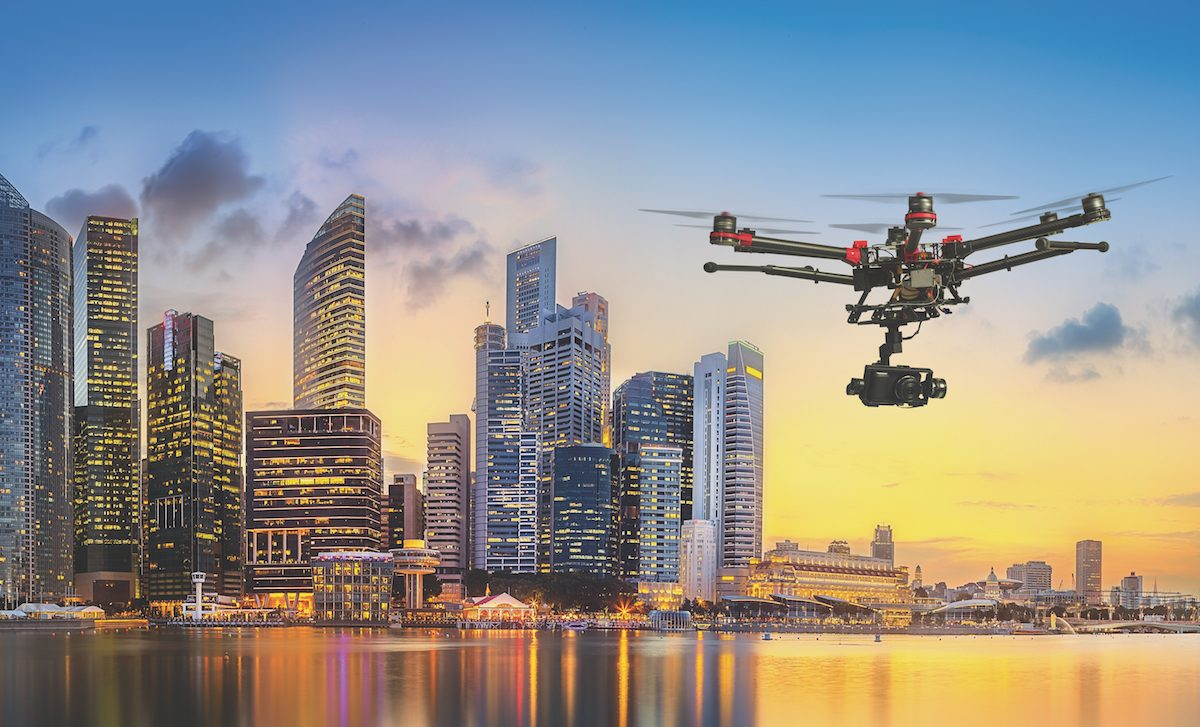
\includegraphics[width=\linewidth]{../Figure/Q1/UAV-on-City.jpg}
	\caption{استفاده از پهپاد جهت عکاسی هوایی
	}
\end{figure}
\subsubsection{اجزای سیستم هدایت}
\begin{itemize}
	\item حسگرهای هدایت
	
	این پهپاد حسگرهای هدایت متنوعی برای فازهای مختلف هدایت دارد. این حسگرها شامل سیستم ناوبری اینرسی
	همراه با سیستم موقعیت یابی جهانی\LTRfootnote{Global Positioning System}
	و ژیروسکوپ\LTRfootnote{Gyro Inertial Measurement Unit}
	است. سایر حسگرهای هدایت شامل دوربین و سونار\LTRfootnote{Sound Navigation and Ranging (Sonar)}
	است.
	\item پردازنده هدایت
	
	با توجه به ماموریت و هدف پردازنده آن می‌تواند خارجی و داخلی باشد.
	\item الگوریتم هدایت
	
	با توجه به هدف (عکاسی هوایی) و یکسان نبودن اهداف در طول زمان، الگوریتم هدایت حلقه بسته است.
	\item تجهیزات مخابراتی
	
	این پرنده تصاویر گرفته شده و یا حتی تصاویر دوربین را به صورت برخط\LTRfootnote{Online} 
	برای اپراتور ارسال کند. برای ارسال و دریافت می‌تواند از تکنولوژی \lr{WiFi}
	استفاده کند.
\end{itemize}


\subsubsection{مراحل هدایت و هدف}
مراحل هدایت این وسیله پرنده، شامل سه فاز آغازین، میانی و پایانی است که هر کدام به اختصار بیان شده است.
\begin{itemize}
	\item فاز آغازین
	
	فاز آغازین را می‌توان به صورت حلقه‌باز در نظر گرفت. در این فاز هدف برخاست\LTRfootnote{Take-Off}
	پرنده و رسیدن به یک ارتفاع معقول جهت انجام هدف است. 
	این فاز نیاز به محاسبات زیادی ندارد و می‌توان فرمان‌ها را به صورت تابعی از زمان اجرا کرد.
	
	\item فاز میانی
	
	به دلیل اینکه فاز توسط اپراتور به‌صورت برخط انجام می‌شود، حلقه بسته است.
	
	\item فاز پایانی
	
	برای نشستن\LTRfootnote{Landing}
	می‌توان به صورت حلقه بسته در نظر گرفت. به این صورت که، پرنده در ارتفاع خاصی که قرار گرفت به صورت حلقه باز ینشیند. برای اینکه پرنده هنگام نشستن ضربه نخورد، به طور معمول از حلقه‌‌بسته استفاده شده است.
\end{itemize}

\subsubsection{انتخاب مسیر هدایت}

در تمامی فازها می‌توان از مسیر هدایت خط دید استفاده کرد. در هر فاز یک خط دید فرضی وجود که پرنده باید آن را دنبال کند. این خط دید ممکن است توسط کامپیوتر پرنده یا اپراتور ساخته شود.
\subsubsection{نوع حسگرهای هدایت}
بر اساس توضیحات ارائه شده دارای حسگر مطلق و نسبی (دوربین) است. می‌توان آشکارساز را چشم اپراتور در نظر گرفت. بنابراین نیمه فعال است.
خروجی حسگرها شامل موقعیت در دستگاه اینرسی و نسبی، فاصله با اجسام،  وضعیت و زاویه سمت است.
\subsubsection{سیستم ناوبری}
در فاز آغازین و پایانی به این دلیل که تنها ارتفاع لازم است، می‌توان آن را اینرسی درنظر گرفت. در فاز میانی از سیستم ناوبری ترکیبی اینرسی و رادیویی استفاده می‌شود. در این فاز اگر از دوربین جهت محاسبه سرعت و مکان استفاده شود، می‌توان ناوبری تصویری را هم به ناوبری ترکیبی اضافه کرد.

\subsubsection{سیستم هدایت}
در دو فاز اول می‌توان به اینرسی اکتفا کرد. در فاز میانی فرمان از اپراتور صادر می‌شود اما فرمان‌هایی مانند ایستادن در ارتفاع ثابت توسط اپراتور ارسال نمی‌شود. این نوع فرمان‌ها را می‌توان اینرسی در نظر گرفت. بنابراین، سیستم هدایت آن ترکیب سیستم‌های هدایت فرمانی و اینرسی است.





















